\begin{exercise}
For an arbitrary category \(\cat{B}\), let \(\cat{B}_{\bullet}^{\rightarrow}\) be the category with \textbf{pointed families} as objects;
these are pairs \(\left\langle\begin{pmatrix}\begin{tikzcd}[row sep=small] X \arrow[d, "\varphi"] \\ I\end{tikzcd}\end{pmatrix}, s\right\rangle\) where \(s\) is a section of \(\varphi\)
(\emph{i.e.} a map \(s : I \to X\) with \(\varphi \circ s = \id\)).
A morphism \(\left\langle\begin{pmatrix}\begin{tikzcd}[row sep=small] X \arrow[d, "\varphi"] \\ I\end{tikzcd}\end{pmatrix}, s\right\rangle \to \left\langle\begin{pmatrix}\begin{tikzcd}[row sep=small] Y \arrow[d, "\psi"] \\ J\end{tikzcd}\end{pmatrix}, t\right\rangle\) in \(\cat{B}_{\bullet}^{\rightarrow}\) consists of a pair of morphisms \(u : I \to J\), \(f : X \to Y\) in \(\cat{B}\) with \(\psi \circ f = u \circ \varphi\) and also \(f \circ s = t \circ u\).
Thus morphisms of pointed families preserve the points (\emph{i.e.} sections) of the families.
Prove that
\begin{parts}
\part
if the category \(\cat{B}\) has pullbacks then the functor \(\cat{B}_{\bullet}^{\rightarrow}\) sending\\\(\left\langle\begin{pmatrix}\begin{tikzcd}[row sep=small] X \arrow[d, "\varphi"] \\ I\end{tikzcd}\end{pmatrix}, s\right\rangle\) to the index set \(I\) is a fibration;
\part
for \(\cat{B} = \Sets\), there is an equivalence of categories \(\Fam(\Sets_{\bullet}) \xrightarrow{\simeq} \Sets_{\bullet}^{\rightarrow}\) like in Proposition~1.2.2, where \(\Sets_{\bullet}\) is the category of \textbf{pointed sets}: objects are sets containing a distinguished base point, morphisms are functions preserving such points.
\end{parts}
\end{exercise}

\begin{partsolution}{i}
Let \(\cat{B}\) be a category with pullbacks, and consider the functor
\begin{equation*}
\begin{tikzcd}[row sep=small]
\cat{B}_{\bullet}^{\rightarrow} \arrow[r] & \cat{B} \\
\left\langle
\begin{pmatrix}
\begin{tikzpicture}
\node(1){\(X\)};
\node(2)[below of=1]{\(I\)};
\draw[->](1)--node[right]{\scriptsize\(\varphi\)} (2);
\end{tikzpicture}
\end{pmatrix}, s\right\rangle
\arrow[ddd, "{(u, f)}"{name=A}] \arrow[r, mapsto]
& I \arrow[ddd, "u"{right}, " "{left, name=B}] \\\\\\
\left\langle
\begin{pmatrix}
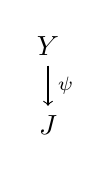
\begin{tikzpicture}
\node(1){\(Y\)};
\node(2)[below of=1]{\(J\)};
\draw[->](1)--node[right]{\scriptsize\(\psi\)} (2);
\end{tikzpicture}
\end{pmatrix}, t\right\rangle
\arrow[r, mapsto] & J 
\arrow[from=A, to=B, mapsto]
\end{tikzcd}
\end{equation*}
where the morphism \((u, f)\) represents the commutative diagram
\begin{equation}
\label{eq:ex:1.2.3.i:morphism}
\begin{tikzcd}
I \arrow[r, "u"] \arrow[d, "s"] \arrow[dd, bend right, "\id_I"{left}] & J \arrow[d, "t"{left}] \arrow[dd, bend left, "\id_J"] \\
X \arrow[r, "f"] \arrow[d, "\varphi"] & Y \arrow[d, "\psi"{left}] \\
I \arrow[r, "u"] & J
\end{tikzcd}
\end{equation}
We claim that \(\cat{B}_{\bullet}^{\rightarrow} \to \cat{B}\) is a fibration.
To this end, let \(u : I \to J\) be a morphism in \(\cat{B}\), and let \(\left\langle\begin{pmatrix}\begin{tikzcd}[row sep=small] Y \arrow[d, "\psi"] \\ J\end{tikzcd}\end{pmatrix}, t\right\rangle\) be an object in \(\cat{B}_{\bullet}^{\rightarrow}\) above \(J\).
Since \(\cat{B}\) has pullbacks, let \(I \xleftarrow{\varphi} X \xrightarrow{f} Y\) be a pullback of \(I \xrightarrow{u} J \xleftarrow{\psi} Y\).
Moreover, define \(s : I \to X\) as the unique dashed arrow that makes the following diagram commute, by virtue of \(I \xleftarrow{\varphi} X \xrightarrow{f} Y\) being a pullback of \(I \xrightarrow{u} J \xleftarrow{\psi} Y\).
\begin{equation*}
\begin{tikzcd}
I \arrow[dr, dashed, "s"] \arrow[ddr, "\id_I"{below left}, bend right] \arrow[r, "u"]
& J \arrow[dr, "t"] \\
& X \arrow[dr, phantom, " "{pullback}, very near start] \arrow[r, "f"] \arrow[d, "\varphi"] & Y \arrow[d, "\psi"] \\
& I \arrow[r, "u"] & J
\end{tikzcd}
\end{equation*}
In particular, \(\varphi \circ s = \id_I\), so \(\left\langle\begin{pmatrix}\begin{tikzcd}[row sep=small] X \arrow[d, "\varphi"] \\ I\end{tikzcd}\end{pmatrix}, s\right\rangle\) is an object in \(\cat{B}_{\bullet}^{\rightarrow}\).
Also, we have a situation as in \eqref{eq:ex:1.2.3.i:morphism}, namely that
\begin{align*}
\psi \circ f &= u \circ \varphi, &
f \circ s = t \circ u,
\end{align*}
so we have a morphism
\begin{equation}
\label{eq:ex:1.2.3.i.lift}
\begin{tikzcd}
\left\langle
\begin{pmatrix}
\begin{tikzpicture}
\node(1){\(X\)};
\node(2)[below of=1]{\(I\)};
\draw[->](1)--node[right]{\scriptsize\(\varphi\)} (2);
\end{tikzpicture}
\end{pmatrix}, s\right\rangle
\arrow[r, "{(u, f)}"] &
\left\langle
\begin{pmatrix}
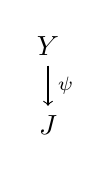
\begin{tikzpicture}
\node(1){\(Y\)};
\node(2)[below of=1]{\(J\)};
\draw[->](1)--node[right]{\scriptsize\(\psi\)} (2);
\end{tikzpicture}
\end{pmatrix}, t\right\rangle
\end{tikzcd}
\end{equation}
in \(\cat{B}_{\bullet}^{\rightarrow}\).
We claim that it is a Cartesian lift of \(u\).
Indeed, consider a morphism \(v : K \to I\) in \(\cat{B}\) and a morphism
\begin{equation*}
\begin{tikzcd}
\left\langle
\begin{pmatrix}
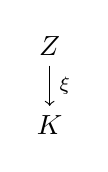
\begin{tikzpicture}
\node(1){\(Z\)};
\node(2)[below of=1]{\(K\)};
\draw[->](1)--node[right]{\scriptsize\(\xi\)} (2);
\end{tikzpicture}
\end{pmatrix}, r\right\rangle
\arrow[r, "{(u \circ v, g)}"] &
\left\langle
\begin{pmatrix}
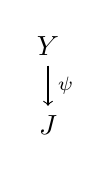
\begin{tikzpicture}
\node(1){\(Y\)};
\node(2)[below of=1]{\(J\)};
\draw[->](1)--node[right]{\scriptsize\(\psi\)} (2);
\end{tikzpicture}
\end{pmatrix}, t\right\rangle
\end{tikzcd}
\end{equation*}
in \(\cat{B}_{\bullet}^{\rightarrow}\) above \(u \circ v\).
These data are summarized by the solid arrows in the following commutative diagram.
\begin{equation}
\label{eq:ex:1.2.3.i:cartesian}
\begin{tikzcd}[row sep=small]
\left\langle
\begin{pmatrix}
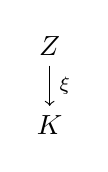
\begin{tikzpicture}
\node(1){\(Z\)};
\node(2)[below of=1]{\(K\)};
\draw[->](1)--node[right]{\scriptsize\(\xi\)} (2);
\end{tikzpicture}
\end{pmatrix}, r\right\rangle
\arrow[rrd, bend left, near end, "{(u \circ v, g)}"]
\arrow[rd, dashed, "?"]
\arrow[dd, -Triangle]
\\[-7ex]
&
\left\langle
\begin{pmatrix}
\begin{tikzpicture}
\node(1){\(X\)};
\node(2)[below of=1]{\(I\)};
\draw[->](1)--node[right]{\scriptsize\(\varphi\)} (2);
\end{tikzpicture}
\end{pmatrix}, s\right\rangle
\arrow[r, "{(u, f)}"]
\arrow[dd, -Triangle]
&
\left\langle
\begin{pmatrix}
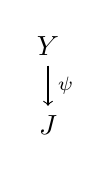
\begin{tikzpicture}
\node(1){\(Y\)};
\node(2)[below of=1]{\(J\)};
\draw[->](1)--node[right]{\scriptsize\(\psi\)} (2);
\end{tikzpicture}
\end{pmatrix}, t\right\rangle
\arrow[dd, -Triangle]
\\
K \arrow[rd, "v"]
\\
& I \arrow[r, "u"] & J
\end{tikzcd}
\end{equation}
We must find a unique filler for the dashed arrow above \(v\) labeled ``\(?\)'' in \eqref{eq:ex:1.2.3.i:cartesian} that makes the diagram commute.
Moreover, the situation in \eqref{eq:ex:1.2.3.i:cartesian} can also be summarized by the following commutative diagram in \(\cat{B}\).
\begin{equation}
\label{eq:ex:1.2.3.i:squares}
\begin{tikzcd}
K \arrow[d, "r"] \arrow[dd, bend right, "\id_K"{left}] \arrow[r, "v"]
& I \arrow[r, "u"] \arrow[d, "s"{near start}]
& J \arrow[d, "t"{left}] \arrow[dd, bend left, "\id_J"]
\\
Z \arrow[d, "\xi"]
& X \arrow[d, "\varphi"] \arrow[r, "f"{below}] \arrow[dr, phantom, " "{pullback}, very near start]
& Y \arrow[d, "\psi"{left}]
\\
K \arrow[r, "v"]
& I \arrow[r, "u"]
& J
\arrow[from=llu, to=u, crossing over, bend left, near end, "g"]
\arrow[from=luu, to=l, crossing over, bend right, "\id_I"{left}]
\end{tikzcd}
\end{equation}
In particular, since \(\psi \circ g = u \circ v \circ \xi\), the universal property of the pullback \(I \xleftarrow{\varphi} X \xrightarrow{f} Y\) implies that there exists a unique morphism \(h : Z \to X\) in \(\cat{B}\) such that the following diagram in \(\cat{B}\) commutes.
\begin{equation*}
\begin{tikzcd}
Z \arrow[dr, dashed, "h"] \arrow[drr, "g", bend left] \arrow[d, "\xi"{left}] \\
K \arrow[dr, "v"{below left}]
& X \arrow[dr, phantom, " "{pullback}, very near start] \arrow[r, "f"] \arrow[d, "\varphi"{left}]
& Y \arrow[d, "\psi"] \\
& I \arrow[r, "u"] & J
\end{tikzcd}
\end{equation*}
Also, since we have both
\begin{align*}
\psi \circ f \circ s \circ v
&= u \circ \varphi \circ s \circ v, \\
\psi \circ f \circ h \circ r
&= \psi \circ g \circ r
= u \circ v \circ \xi \circ r
= u \circ \varphi \circ h \circ r,
\end{align*}
the universal property of the pullback \(I \xleftarrow{\varphi} X \xrightarrow{f} Y\) implies that \(s \circ v = h \circ r\), as in the following commutative diagram in \(\cat{B}\).
\begin{equation*}
\begin{tikzcd}
K \arrow[dr, bend left, "s \circ v", " "{below left, name=A}] \arrow[dr, bend right, "h \circ r"{below left}, " "{above right, name=B}] \\
& X \arrow[dr, phantom, " "{pullback}, very near start] \arrow[r, "f"] \arrow[d, "\varphi"{left}] & Y \arrow[d, "\psi"] \\
& I \arrow[r, "u"] & J
\arrow[from=A, to=B, equal]
\end{tikzcd}
\end{equation*}
Thus, \eqref{eq:ex:1.2.3.i:squares} can be extended into the following commutative diagram.
\begin{equation*}
\begin{tikzcd}
K \arrow[d, "r"] \arrow[dd, bend right, "\id_K"{left}] \arrow[r, "v"]
& I \arrow[r, "u"] \arrow[d, "s"{near start}]
& J \arrow[d, "t"{left}] \arrow[dd, bend left, "\id_J"]
\\
Z \arrow[d, "\xi"]
& X \arrow[d, "\varphi"] \arrow[r, "f"{below}] \arrow[dr, phantom, " "{pullback}, very near start]
& Y \arrow[d, "\psi"{left}]
\\
K \arrow[r, "v"]
& I \arrow[r, "u"]
& J
\arrow[from=llu, to=u, crossing over, bend left, near end, "g"]
\arrow[from=luu, to=l, crossing over, bend right, near end, "\id_I"{below left}]
\arrow[from=llu, to=ul, crossing over, "h"{below}]
\end{tikzcd}
\end{equation*}
It follows that one choice of ``\(?\)'' filler in \eqref{eq:ex:1.2.3.i:cartesian} is \(? = (v, h)\), and its uniqueness follows from the uniqueness of \(h\) since \(I \xleftarrow{\varphi} X \xrightarrow{f} Y\) is a pullback.
Thus, \eqref{eq:ex:1.2.3.i.lift} is Cartesian, and hence \(\cat{B}_{\bullet}^{\rightarrow} \to \cat{B}\) is a fibration.
\end{partsolution}

\begin{partsolution}{ii}
We define functors
\begin{align*}
F &: \Fam(\Sets_{\bullet}) \to \Sets_{\bullet}^{\rightarrow}, &
G &: \Sets_{\bullet}^{\rightarrow} \to \Fam(\Sets_{\bullet})
\end{align*}
on objects by
\begin{equation*}
F\left(\left(X_i, x_i\right)_{i \in I}\right)
= \left\langle\begin{pmatrix}
\begin{tikzcd}[row sep=small]
\sum_{i \in I} X_i \arrow[d, "\fst"] \\ I
\end{tikzcd}
\end{pmatrix}, i \mapsto x_i\right\rangle
\end{equation*}
and
\begin{equation*}
G\left(\left\langle
\begin{pmatrix}
\begin{tikzcd}[row sep=small]
X \arrow[d, "\varphi"] \\ I
\end{tikzcd}
\end{pmatrix}, s
\right\rangle\right)
= \left(\varphi^{-1}(\{i\}), s(i)\right)_{i \in I}
\end{equation*}
and on morphisms by
\begin{equation*}
F\left(\left(X_i, x_i\right)_{i \in I} \xrightarrow{(u, f)} \left(Y_j, y_j\right)_{j \in J}\right)
= \big(u, (i, x) \mapsto (u(i), f_i(x))\big)
\end{equation*}
and
\begin{equation*}
G\left(
\left\langle
\begin{pmatrix}
\begin{tikzcd}[row sep=small]
X \arrow[d, "\varphi"] \\ I
\end{tikzcd}
\end{pmatrix}, s
\right\rangle
\xrightarrow{(u, f)}
\left\langle
\begin{pmatrix}
\begin{tikzcd}[row sep=small]
Y \arrow[d, "\psi"] \\ J
\end{tikzcd}
\end{pmatrix}, t
\right\rangle
\right)
= \left(u, \left(f|_{\varphi^{-1}(\{i\})}\right)_{i \in I}\right).
\end{equation*}
Then we have
\begin{align*}
G\left(F\left(\left(X_i, x_i\right)_{i \in I}\right)\right)
&= \big(\{i\} \times X_i, x_i\big)_{i \in I}
\cong \left(X_i, x_i\right)_{i \in I}, \\
F\left(G\left(\left\langle
\begin{pmatrix}
\begin{tikzcd}[row sep=small]
X \arrow[d, "\varphi"] \\ I
\end{tikzcd}
\end{pmatrix}, s
\right\rangle\right)\right)
&= \left\langle
\begin{pmatrix}
\begin{tikzcd}[row sep=small]
\sum_{i\in I} \varphi^{-1}(\{i\}) \arrow[d, "\fst"] \\ I
\end{tikzcd}
\end{pmatrix}, s
\right\rangle
\cong \left\langle
\begin{pmatrix}
\begin{tikzcd}[row sep=small]
X \arrow[d, "\varphi"] \\ I
\end{tikzcd}
\end{pmatrix}, s
\right\rangle.
\end{align*}
We omit the proofs of the  naturality of these isomorphisms, and conclude that \(G \circ F \cong \id_{\Fam(\Sets_{\bullet})}\) and \(F \circ G \cong \id_{\Sets_{\bullet}^{\rightarrow}}\), and that, in particular, there is an equivalence of categories \(F : \Fam(\Sets_{\bullet}) \xrightarrow{\simeq} \Sets_{\bullet}^{\rightarrow}\)
\end{partsolution}